% !TEX program = lualatex
%
% Final-presentation template, styled after the i6 (Chair of Machine Learning
% and Reasoning, RWTH Aachen) final-talk deck.  It reuses the thesis fonts
% (Noto Sans + STIX Two Math) and the RWTH logo from ../graphics, so it
% compiles with the same toolchain as the thesis:
%
%     cd thesis/presentation
%     latexmk -pdf -lualatex -interaction=nonstopmode presentation.tex
%
% ---------------------------------------------------------------------------
% TO FILL IN: search for the word  FILL  below.  At minimum, edit the title /
% author / date block and replace the placeholder bullets on each content
% slide.  Everything else (colours, logos, footer, layout) already matches.
% ---------------------------------------------------------------------------

\documentclass[aspectratio=169, 11pt]{beamer}

% --- fonts: NotoSans body (matches the thesis) + classic serif math ---------
% Note: we deliberately do NOT load unicode-math here. In beamer it clashes
% with \setsansfont under TeX Live 2026 (a fatal "cannot find file ''" at
% shutdown). Math therefore uses the default serif math font, which is the
% right look for slides anyway.
\usefonttheme{professionalfonts}     % keep math serif; don't let beamer sans-ify it
\usepackage{fontspec}
% Ligatures=NoCommon: this NotoSans build has a broken "fi" ligature glyph (it
% renders as "ß"). In the thesis it never shows because the body font there is
% serif STIX; here the body IS NotoSans, so we disable the common ligatures.
\setmainfont{NotoSans}[
  Extension=.ttf, Path=../fonts/, Ligatures=NoCommon,
  UprightFont={*-Regular}, BoldFont={*-Bold},
  ItalicFont={*-Italic}, BoldItalicFont={*-BoldItalic}]
\setsansfont{NotoSans}[
  Extension=.ttf, Path=../fonts/, Ligatures=NoCommon,
  UprightFont={*-Regular}, BoldFont={*-Bold},
  ItalicFont={*-Italic}, BoldItalicFont={*-BoldItalic}]
\setmonofont{NotoSansMono}[
  Extension=.ttf, Path=../fonts/, Ligatures=NoCommon,
  UprightFont={*-Regular}, BoldFont={*-Bold}]

% Emoji (future-work slide). LuaLaTeX only; Noto Color Emoji isn't installed on
% this machine, so point the emoji package at the Windows Segoe UI Emoji font
% (COLR/CPAL colour, rendered via Harfbuzz).
\usepackage{emoji}
\setemojifont{Segoe UI Emoji}[Renderer=Harfbuzz]

\usepackage{tikz}
\usetikzlibrary{positioning, arrows.meta, overlay-beamer-styles, calc}
\usepackage{booktabs}
\usepackage{graphicx}
\graphicspath{{../graphics/}{../graphics/titlepage/}}

% --- colours ---------------------------------------------------------------
\definecolor{i6blue}{RGB}{20,33,200}   % frame titles, bullets, accents
\definecolor{i6teal}{RGB}{17,138,131}  % the ML&R logo nodes
\definecolor{bodygray}{RGB}{64,68,82}  % body text

% --- look & feel -----------------------------------------------------------
\setbeamertemplate{navigation symbols}{}
\setbeamercolor{normal text}{fg=bodygray}
\setbeamercolor{frametitle}{fg=i6blue}
\setbeamerfont{frametitle}{series=\bfseries, size=\large}
\setbeamercolor{structure}{fg=i6blue}          % itemize markers + enumerate numbers
\setbeamercolor{itemize item}{fg=i6blue}
\setbeamercolor{itemize subitem}{fg=i6blue}
\setbeamercolor{itemize subsubitem}{fg=i6blue}
\setbeamertemplate{itemize items}[triangle]
\setbeamercolor{title}{fg=i6blue}
\setbeamercolor{subtitle}{fg=i6blue}
\setbeamertemplate{section in toc}[sections numbered]
\setbeamercolor{section number projected}{bg=white, fg=i6blue}

% footer:  "Author: running title" on the left, frame number on the right
\setbeamertemplate{footline}{%
  \hbox{\begin{beamercolorbox}[wd=\paperwidth, ht=3ex, dp=1.6ex,
        leftskip=4mm, rightskip=4mm]{}%
    {\color{gray}\insertshortauthor:}\,%
    {\color{i6blue!55}\insertshorttitle}%
    \hfill{\color{gray}\insertframenumber}%
  \end{beamercolorbox}}%
}

% Title-slide logo bar. The thesis ships the official combined logo
% (i6 ML&R chair mark + "Chair of Machine Learning and Reasoning" + RWTH
% wordmark) as one PDF, which is exactly the bar used in the reference deck.
\newcommand{\titlelogos}{
\includegraphics[height=17mm]{rwth-logo}}

% a blue bold in-frame sub-heading (e.g. "Example ...") like the reference deck
\newcommand{\subhead}[1]{{\color{i6blue}\bfseries #1}\par\medskip}

% \stepline{<overlay-spec>}{text}: colour a pseudocode line i6blue on the given
% overlay(s) -- e.g. \stepline{2}{...} or \stepline{4-5}{...}. Drives the
% highlight in the boxelization algorithm walkthrough.
\newcommand{\stepline}[2]{\alt<#1>{{\color{i6blue}#2}}{#2}}

% \rc{Author et al.}{Alpha-key}: an inline reference in the i6 reference-deck
% style -- "(Author et al. [Key])" with the alphabetic key (biblatex
% alphabetic, maxalphanames=1) set small and in muted blue. The slides carry no
% bibliography, so citations are written by hand against thesis/resources/references.bib.
\newcommand{\rc}[2]{{\footnotesize\,(#1\;{\color{i6blue!60}[#2]})}}

% ---------------------------------------------------------------------------
% FILL: talk metadata
% ---------------------------------------------------------------------------
% The text in [..] is the short title shown in the footer; the {..} is the
% full title shown on the title slide (use \\ to break it across two lines).
\title[Semantic Space Abstractions for POD-TAMP]%
      {Semantic Space Abstractions for Partially Observable\\Deterministic Task and Motion Planning}
\subtitle{Final Presentation}
\author[Hani]{Hani Alassiri Alhabboub}
\newcommand{\talkdate}{23\textsuperscript{rd} Jun, 2026}   % FILL: defence date

\begin{document}

% ===========================================================================
% Title slide
% ===========================================================================
\begin{frame}[plain]
  \vfill
  \begin{center}
    % Font sizes chosen to match the i6 reference deck (GOOD MT.pdf).
    {\fontsize{12}{15}\selectfont\color{i6blue}\inserttitle\par}
    \medskip
    {\fontsize{9.2}{11}\selectfont\color{i6blue}\insertsubtitle\par}
    \vspace{11mm}
    {\fontsize{9.2}{11}\selectfont\color{bodygray}\insertauthor\par}
    \vspace{9mm}
    {\fontsize{9}{11}\selectfont\color{gray}\talkdate\par}
    \vspace{13mm}
    \titlelogos
  \end{center}
  \vfill
\end{frame}

% ===========================================================================
% Roadmap (table of contents)
% ===========================================================================
\begin{frame}{Roadmap}
  \vspace{4mm}
  \tableofcontents
\end{frame}

% ===========================================================================
% 1. Introduction
% ===========================================================================
\section{Introduction}

% Tip: the `[<+->]' overlay spec reveals one bullet per click, just like the
% reference deck.  Use it on every list you want to build up step by step.
% This is a DRAFT grounded in your intro chapter -- tighten the wording to taste.

% --- 1. Motivation (text only, build-up) ---
\begin{frame}{Introduction}
  \begin{itemize}[<+->]
    \item Goal: robots that carry out everyday tasks on their own --- fetch an
          object, clear a table
    \item This needs both multi-step reasoning \emph{and} physical manipulation
          $\Rightarrow$ \textbf{Task and Motion Planning (TAMP)}
    \item TAMP links a high-level goal to feasible motion: a symbolic task plan,
          checked against geometry and kinematics
    \item \textbf{But}: classical TAMP (such as PDDLStream) assumes a
          \emph{fully observable}, \emph{deterministic} world
  \end{itemize}
\end{frame}

% --- 2. The problem + research question (hero scene) ---
\begin{frame}{Introduction: Planning under Occlusion}
  \begin{columns}[T]
    \begin{column}{0.52\textwidth}
      \begin{itemize}[<+->]
        \item Real scenes are \textbf{partially observable}: occlusion, limited
              sensor coverage
        \item The target can be hidden --- the robot must \emph{look} before it
              can act
        \item It needs a \textbf{belief} over where hidden objects are
        \item A uniform voxel grid is the obvious way to represent it ---
              but it \textbf{blows up} $\Rightarrow$ too slow to plan
      \end{itemize}
    \end{column}
    \begin{column}{0.46\textwidth}
      \centering
      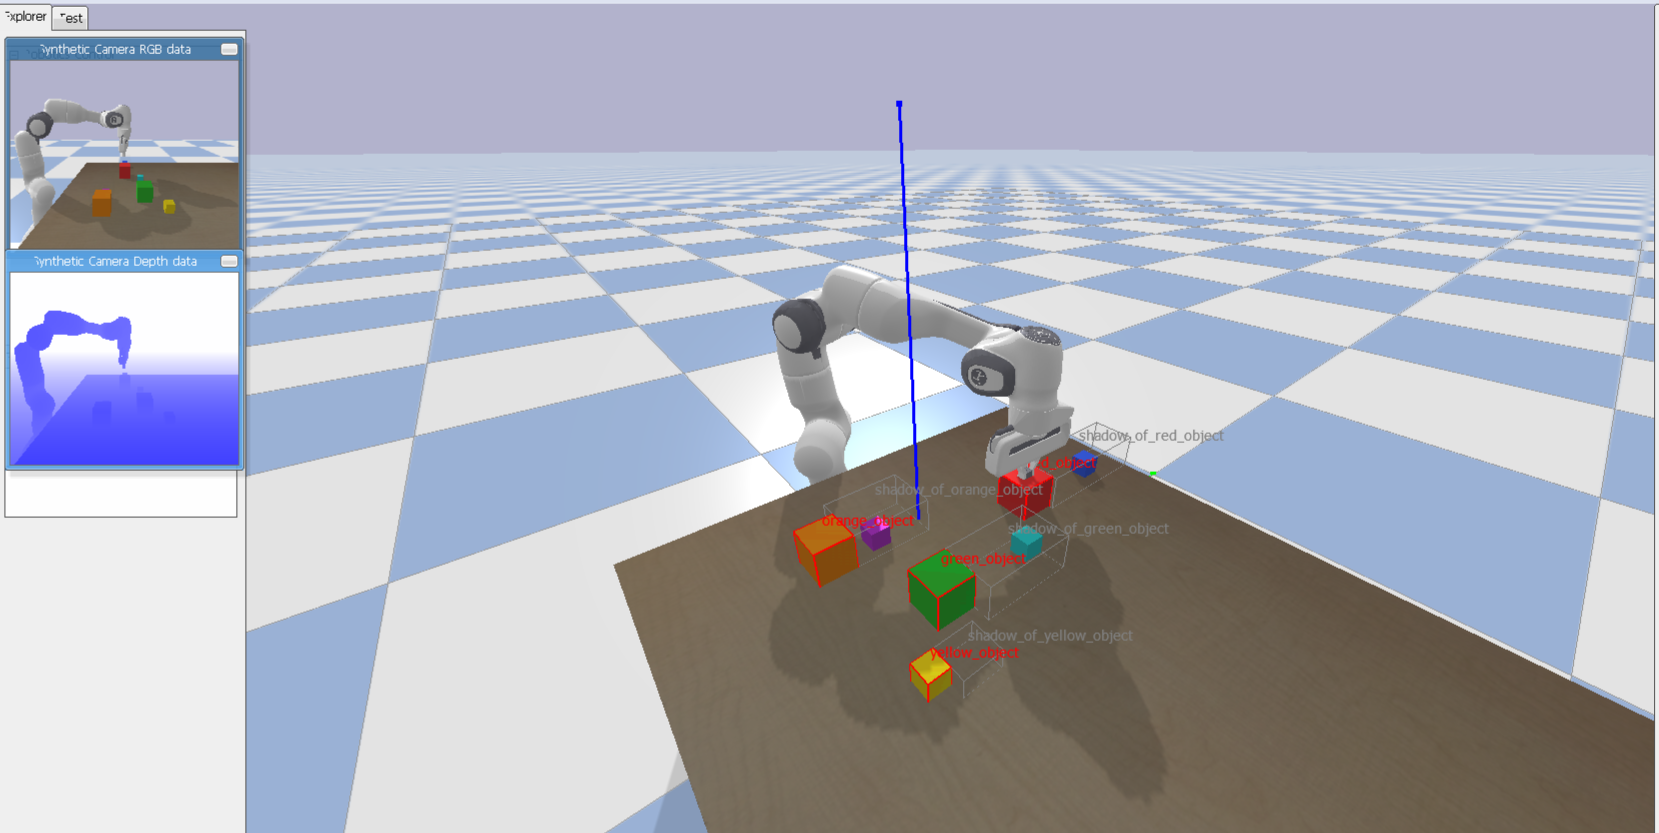
\includegraphics[width=\linewidth]{sim/scene_hidden_target.png}\\[2pt]
      {\footnotesize\color{gray} Target (cyan) hidden behind the green cube;
       one fixed camera (RGB/depth insets).}
    \end{column}
  \end{columns}
  \vspace{2mm}
  \onslide<+->{%
  {\color{i6blue}\textbf{Research question:}} How can we define and integrate a
  belief representation based on \emph{semantic partitioning} into a partially
  observable deterministic (POD) TAMP framework?}
\end{frame}

% --- 3. The idea + contributions (3D Boxel figure as teaser) ---
\begin{frame}{Introduction: The Boxel Idea}
  \begin{columns}[T]
    \begin{column}{0.52\textwidth}
      \begin{itemize}[<+->]
        \item \textbf{Idea}: put the structure of space into the symbolic
              planning state
        \item The \textbf{Boxel} --- a \emph{box-shaped cell} of the workspace
              that either
              \begin{itemize}[<+->]
                \item bounds a detected object,
                \item marks the region it \emph{occludes} (shadow), or
                \item covers free space
              \end{itemize}
        \item Fine where it matters, coarse elsewhere --- a handful of cells,
              not a dense grid
        \item A classical planner reasons over these few cells, and \emph{looks}
              only where it must
      \end{itemize}
    \end{column}
    \begin{column}{0.46\textwidth}
      \centering
      \only<-2>{\includegraphics[width=\linewidth]{boxel_stage_scene.png}}%
      \only<3>{\includegraphics[width=\linewidth]{boxel_stage_object.png}}%
      \only<4>{\includegraphics[width=\linewidth]{boxel_stage_shadow.png}}%
      \only<5->{\includegraphics[width=\linewidth]{boxel_stage_free.png}}%
      \\[1pt]
      {\footnotesize\color{gray} Full construction in the Approach section.}
    \end{column}
  \end{columns}
\end{frame}

% ===========================================================================
% 2. Background
% ===========================================================================
\section{Background}

% --- B1. Classical planning / PDDL ---
\begin{frame}{Background: Classical Planning}
  \begin{itemize}[<+->]
    \item A planning problem $P$: reach a \textbf{goal} from an \textbf{initial
          state} by choosing \textbf{actions} --- captured by its \textbf{state
          model} $S(P)$
  \end{itemize}
  \onslide<+->{%
  \begin{equation*}
    S(P) \;=\; \langle\, S,\; s_0,\; S_G,\; Act,\; A,\; f \,\rangle
  \end{equation*}}
  {\footnotesize
   \only<+->{states $S$}%
   \only<+->{; initial state $s_0$}%
   \only<+->{; goal states $S_G\subseteq S$}%
   \only<+->{; actions $Act$}%
   \only<+->{; $A(s)$, the actions applicable in $s$}%
   \only<+->{; and the deterministic transition $s' = f(a,s)$.}%
   \par\smallskip}
  \begin{itemize}[<+->]
    \item \textbf{STRIPS / PDDL} represents it compactly: a \emph{factored} state
          is the set of true atoms, e.g.\
          $\{\texttt{(on A B)},\,\texttt{(handempty)}\}$; an action has
          preconditions and add\,/\,delete effects
  \end{itemize}
\end{frame}

% --- B1b. Heuristic search, with a small search-tree illustration ---
\begin{frame}{Background: Solving It --- Heuristic Search}
  \begin{columns}[T]
    \begin{column}{0.55\textwidth}
      \begin{itemize}[<+->]
        \item Expand states \textbf{best-first}, ordered by a \emph{heuristic}
              $h(s)$ --- an estimate of the remaining distance to the goal
        \item Promising states go first, so the goal is reached \textbf{without
              enumerating} the whole state space
      \end{itemize}
    \end{column}
    \begin{column}{0.45\textwidth}
      \centering
      \begin{tikzpicture}[>=Stealth, font=\scriptsize,
          n/.style ={circle, draw=gray!55, text=gray!75, minimum size=6.5mm, inner sep=0pt},
          on/.style={circle, draw=i6blue, fill=i6blue!12, text=i6blue,
                     line width=1pt, minimum size=6.5mm, inner sep=0pt},
          gn/.style={circle, draw=i6teal, fill=i6teal!18, text=i6teal,
                     line width=1pt, minimum size=6.5mm, inner sep=0pt},
          oe/.style={draw=i6blue, line width=1pt},
          fe/.style={draw=gray!45}]
        \node[on] (s0) {$s_0$};
        \node[n,  below left=9mm and 12mm of s0] (b) {4};
        \node[on, below=9mm of s0] (a) {2};
        \node[n,  below right=9mm and 12mm of s0] (c) {5};
        \draw[fe] (s0)--(b); \draw[oe] (s0)--(a); \draw[fe] (s0)--(c);
        \node[on, below=9mm of a] (d) {1};
        \node[n,  below right=9mm and 11mm of a] (e) {3};
        \draw[oe] (a)--(d); \draw[fe] (a)--(e);
        \node[gn, below=9mm of d] (g) {G};
        \draw[oe] (d)--(g);
        \node[gray!60, below=1.5mm of b] {$\vdots$};
        \node[gray!60, below=1.5mm of c] {$\vdots$};
        \node[gray!60, below=1.5mm of e] {$\vdots$};
      \end{tikzpicture}\\[2pt]
      {\footnotesize\color{gray} Labels: heuristic $h$. Lowest-$h$ path in blue;
       grey branches are never expanded.}
    \end{column}
  \end{columns}
\end{frame}

% --- B2a. Partial observability + belief, built up with a worked example ---
\begin{frame}{Background: When the World Is Not Fully Known}
  \begin{itemize}[<+->]
    \item Unlike classical planning, a robot rarely knows the \textbf{exact state}:
          it cannot see \emph{behind} an object, so it cannot tell where a hidden
          object is --- \textbf{partial observability}
    \item So it holds a \textbf{belief}: the set of world states still consistent
          with what it has seen; \textbf{sensing} shrinks it
  \end{itemize}
  \vspace{1mm}
  \onslide<+->{%
   \centering
   {\footnotesize Example --- a target hidden behind one of three objects:}\\[1.5mm]
   \begin{tikzpicture}[font=\footnotesize, >=Stealth,
       bel/.style={draw=i6blue, rounded corners=3pt, fill=i6blue!6, text=bodygray,
                   align=left, inner sep=5pt},
       lbl/.style={text=i6blue, font=\scriptsize}]
     \node[bel] (b0) {target behind A\\target behind B\\target behind C};
     \node[lbl, above=0.5mm of b0] {belief $b_0$ (3 worlds)};
     \node[bel, right=34mm of b0] (b1) {target behind B\\target behind C};
     \node[lbl, above=0.5mm of b1] {belief $b_1$ (2 worlds)};
     \draw[->, i6blue, line width=0.8pt] (b0) -- (b1)
        node[midway, above, lbl, align=center] {look behind $A$:\\not there};
   \end{tikzpicture}}
\end{frame}

% --- B2b. Knowledge in the state via Know-If fluents, with a worked example ---
% Built up over 6 overlays: (1) value fluent, (2) Know-If fluent, (3) the
% "before" state, (4) the sensing transition, (5) the "after" state, (6) the
% compile-to-classical takeaway. The value fluent is introduced *before* the
% Know-If fluent, and the diagram keeps the value box above the KIF box in each
% state, so the reading is always "the answer, and whether we know it yet".
\begin{frame}{Background: Compiling Knowledge into Classical Planning}
  \vspace{1mm}
  \begin{itemize}
    \item<1-> A \textbf{value fluent} \texttt{obj\_at\_boxel(cup,B)} alone is
          ambiguous: a bare \texttt{(not ...)} can't tell ``looked, it's empty''
          from ``never looked''
    \item<2-> A \textbf{Know-If fluent} \texttt{obj\_at\_boxel\_KIF(cup,B)} adds the
          missing bit --- \emph{is the value known yet?} \rc{Petrick \& Bacchus}{Pet+02}
  \end{itemize}
  \vspace{1mm}
  \onslide<3->{\centering{\color{i6blue}\bfseries Example --- ``is the cup in
   region $B$?''}\par}
  \vspace{1.5mm}
  \centering
  \begin{tikzpicture}[font=\scriptsize, >=Stealth,
      val/.style ={draw=i6blue!55, rounded corners=2pt, fill=white,
                   text=bodygray, font=\ttfamily\scriptsize,
                   inner sep=3pt, text width=40mm, align=left},
      valk/.style={draw=i6blue!55, rounded corners=2pt, fill=white,
                   text=bodygray, font=\ttfamily\scriptsize,
                   inner sep=3pt, text width=40mm, align=left},
      kif/.style ={draw=gray!45, rounded corners=2pt, fill=gray!8,
                   text=gray!70, font=\ttfamily\scriptsize,
                   inner sep=3pt, text width=40mm, align=left},
      kifk/.style={draw=i6blue, rounded corners=2pt, fill=i6blue!12,
                   text=i6blue, font=\ttfamily\scriptsize,
                   inner sep=3pt, text width=40mm, align=left},
      badU/.style={draw=gray!55, fill=gray!12, text=gray!70,
                   rounded corners=2pt, font=\bfseries\scriptsize, inner sep=3pt},
      badK/.style={draw=i6teal, fill=i6teal!15, text=i6teal,
                   rounded corners=2pt, font=\bfseries\scriptsize, inner sep=3pt},
      ttl/.style ={text=i6blue, font=\itshape\scriptsize}]
    % ----- BEFORE sensing (value fluent on top, Know-If below) -----
    \node[ttl, visible on=<3->] (t0) {before sensing $B$};
    \node[val, visible on=<3->, below=1.4mm of t0] (v0)
        {obj\_at\_boxel(cup,B)\\= ?\ \ \textrm{(don't read it yet)}};
    \node[kif, visible on=<3->, below=1.2mm of v0] (k0)
        {obj\_at\_boxel\_KIF(cup,B)\\absent};
    \node[badU, visible on=<3->, below=1.6mm of k0] (s0) {value UNKNOWN};
    % ----- AFTER sensing -----
    \node[valk, visible on=<5->, right=20mm of v0] (v1)
        {obj\_at\_boxel(cup,B)\\= true / false\ \ \textrm{(settled)}};
    \node[ttl, visible on=<5->, above=1.4mm of v1] (t1) {after sensing $B$};
    \node[kifk, visible on=<5->, below=1.2mm of v1] (k1)
        {obj\_at\_boxel\_KIF(cup,B)\\holds};
    \node[badK, visible on=<5->, below=1.6mm of k1] (s1) {value KNOWN};
    % ----- transition arrow -----
    \draw[->, i6blue, line width=1pt, visible on=<4->] (v0.east) -- (v1.west)
        node[midway, above=0.5mm, text=i6blue, font=\scriptsize] {sense $B$}
        node[midway, below=0.5mm, text=i6blue!70, font=\tiny, align=center]
            {sets KIF,\\settles value};
  \end{tikzpicture}
  \par\vspace{1.5mm}
  \onslide<6->{\footnotesize
   This \textbf{compiles} partial observability into a \textbf{classical} problem:
   the planner now seeks a \emph{state of knowledge} --- the target's region
   becomes \emph{known} \rc{Geffner \& Bonet}{Gef+13}.}
\end{frame}

% --- B2c. What kind of uncertainty? (POMDP vs POD) --- placed after the Know-If
% mechanism so it reads as "here is where our approach sits", not a detour ---
\begin{frame}{Background: What Kind of Uncertainty?}
  \vspace{1mm}
  Two very different reasons a plan can be uncertain:
  \begin{itemize}[<+->]
    \item \textbf{Random outcomes} --- e.g.\ a move that occasionally slips
          sideways. This needs a \textbf{POMDP}: a probability distribution over
          states and a \emph{policy} --- expressive, but computationally very
          demanding \rc{Kaelbling et al.}{Kae+98}
    \item \textbf{Missing knowledge} --- the world is fixed and predictable; the
          robot simply cannot \emph{see} where the target is. This needs only to
          track what is \textbf{known vs.\ unknown} --- partially observable
          \emph{deterministic} (POD) planning \rc{Geffner \& Bonet}{Gef+13}
  \end{itemize}
  \vspace{1mm}
  \onslide<+->{%
   {\color{i6blue}\bfseries Ours is the second kind:} the robot's actions are
   reliable --- the only uncertainty is occlusion. So no probabilities; we track
   knowledge, and sensing resolves it.}
\end{frame}

% --- B3. TAMP + PDDLStream, grounded with a concrete pick example ---
\begin{frame}{Background: TAMP and PDDLStream}
  \begin{itemize}[<+->]
    \item So far we have planned over \emph{discrete} symbols --- but every action
          also needs \emph{feasible motion}: TAMP's
          \emph{symbolic\,$\leftrightarrow$\,continuous} gap
    \item \textbf{PDDLStream} adds \textbf{streams}: samplers called \emph{on
          demand} that produce continuous values (a grasp, an IK configuration, a
          path) and \textbf{certify} them as PDDL facts \rc{Garrett et al.}{Gar+18}
  \end{itemize}
  \vspace{0.5mm}
  \onslide<+->{%
  {\color{i6blue}\bfseries Example --- our \texttt{pick} action:}
  \begin{columns}[T]
    \begin{column}{0.57\textwidth}
      {\scriptsize\ttfamily
       (:action pick :parameters (?o ?b ?g ?q)\\
       \hspace*{2mm}:precondition (and (handempty)\\
       \hspace*{8mm}(obj\_at\_boxel ?o ?b)\\
       \hspace*{8mm}(at\_config ?q)\hfill{\rmfamily\color{gray}\itshape\,// from move}\\
       \hspace*{8mm}{\color{i6blue}(Grasp ?g)}\hfill{\rmfamily\color{gray}\itshape\,// sample-grasp}\\
       \hspace*{8mm}{\color{i6blue}(kin\_solution ?o ?b ?g ?q)}))\\
       \hspace*{2mm}:effect (and (holding ?o) ...))\\
      }
    \end{column}
    \begin{column}{0.43\textwidth}
      \centering
      \begin{tikzpicture}[font=\scriptsize, >=Stealth,
          s/.style={draw=i6blue, rounded corners=2pt, fill=white, text=bodygray,
                    font=\ttfamily\scriptsize, inner sep=2.5pt, minimum width=18mm},
          a/.style={draw=i6blue, rounded corners=2pt, fill=i6blue!12, text=i6blue,
                    font=\bfseries, inner sep=4pt},
          cf/.style={font=\ttfamily\tiny, text=i6blue}]
        \node[s] (sg) {sample-grasp};
        \node[s, below=9mm of sg] (ck) {compute-kin};
        \node[a] (pick) at ($(sg)!0.5!(ck) + (24mm,0)$) {pick};
        \draw[->, i6blue, line width=0.8pt] (sg.east) -- (pick.north west)
            node[cf, pos=0.52, above, sloped] {(Grasp ?g)};
        \draw[->, i6blue, line width=0.8pt] (ck.east) -- (pick.south west)
            node[cf, pos=0.52, below, sloped] {(kin\_solution)};
      \end{tikzpicture}\\[3pt]
      {\scriptsize\color{gray} Each stream certifies one \textcolor{i6blue}{blue}
       fact \texttt{pick} needs. The trajectory stream \texttt{plan-motion} feeds
       the preceding \texttt{move}, which sets \texttt{at\_config}.}
    \end{column}
  \end{columns}}
\end{frame}

% ===========================================================================
% 3. Related Work
% ===========================================================================
\section{Related Work}

% Two axes the thesis sits between: how space is represented, and how TAMP
% handles partial observability. Build to the gap at the bottom.
% --- RW1. TAMP under partial observability (the closest comparison; TAMPURA is
% our baseline) ---
\begin{frame}{Related Work: TAMP under Partial Observability}
  \begin{itemize}[<+->]
    \item \textbf{POMDP-based} (TAMPURA): learns an abstract MDP and solves it
          with LAO* --- proactive, but probabilistic and sub-symbolic
          \rc{Curtis et al.}{Cur+24}
    \item \textbf{Reactive, partially-grounded plans}: defer uncertainty to
          execution; no probabilities, but cannot plan multi-step sensing
          \rc{Pan et al.}{Pan+24}
    \item \textbf{Belief from foundation models}: a VLM\,/\,LLM estimates where
          objects are \rc{Zhao et al.}{Zha+25}
    \item \textbf{Determinize-and-replan}: FF-Replan does this for probabilistic
          MDPs \rc{Yoon et al.}{Yoo+07}; the \textbf{K-replanner} does it for
          partial observability via knowledge literals \rc{Bonet \& Geffner}{Bon+11}.
          We keep its replanning idea but \emph{join it to TAMP} on named
          \textbf{Boxel} volumes --- the K-replanner stays purely symbolic, with
          no geometry
  \end{itemize}
\end{frame}

% --- RW2. Spatial representations (the axis the thesis contributes on); builds
% straight into the gap, which is itself about representation ---
\begin{frame}{Related Work: Spatial Representations under Occlusion}
  {\color{i6blue}\textbf{What we look for:}} occlusion as \emph{named, symbolic
  state} a planner can resolve.
  \smallskip
  \begin{columns}[T]
    \begin{column}{0.58\textwidth}
      {\small
      \begin{itemize}[<+->]
        \item \textbf{Octree maps} (OctoMap): map \emph{where matter is};
              unobserved space is only absent evidence, and subdivision is
              geometric, not semantic \rc{Hornung et al.}{Hor+13}
        \item \textbf{Learned critical regions}: abstract space by \emph{task
              relevance}, but predicted once per scene and carry no occlusion
              \rc{Molina et al.}{Mol+20}
        \item \textbf{Occlusion-aware planners}: keep occlusion in a
              \emph{probabilistic belief} (visibility grid or pose distribution),
              not a named volume \rc{Garrett et al.}{Gar+20}
      \end{itemize}}
    \end{column}
    \begin{column}{0.42\textwidth}
      \centering
      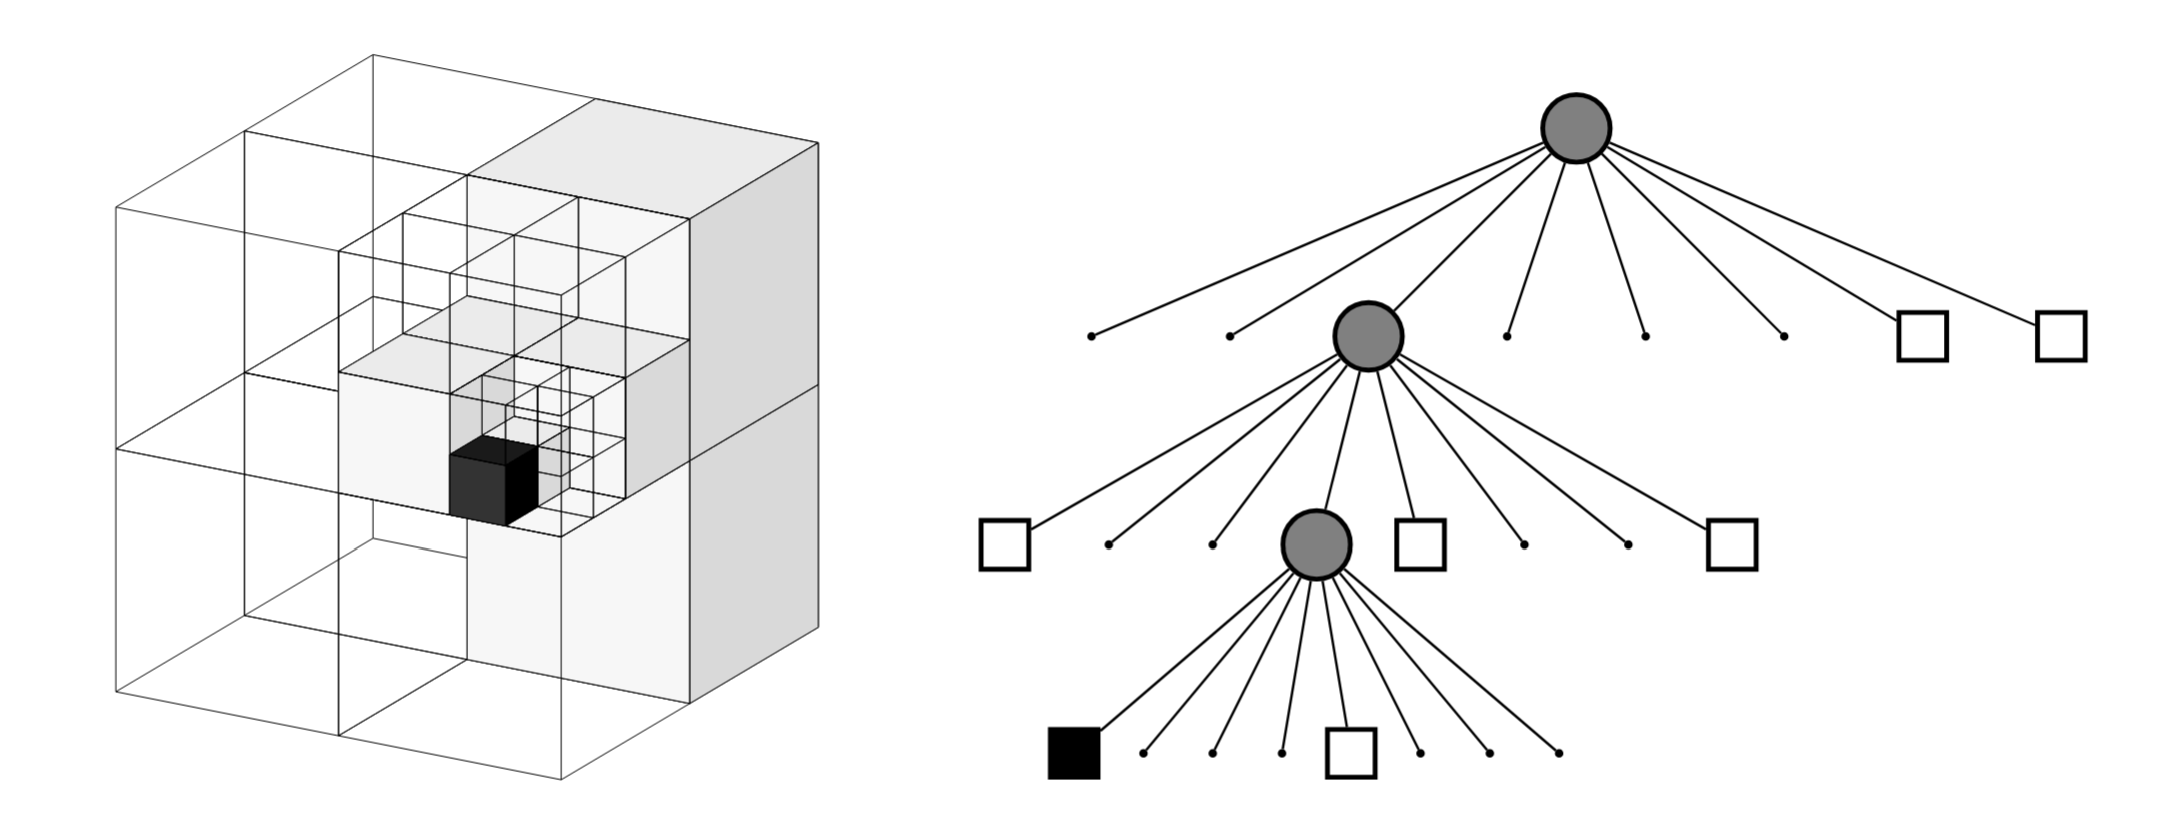
\includegraphics[width=\linewidth]{octmap_illustration.png}\\[3pt]
      {\footnotesize\color{gray} An octree map: free (white) and occupied (black)
       cells, with its tree (after Hornung et al.).}
    \end{column}
  \end{columns}
  \vspace{1mm}
  \onslide<+->{{\color{i6blue}\textbf{The gap:}} none names the occluded
   \emph{volume} as symbolic state that sensing resolves inside a PDDLStream TAMP
   loop --- what this thesis fills.}
\end{frame}

% ===========================================================================
% 4. Approach
% ===========================================================================
\section{Approach}

% --- A1. Method overview: the Sense--Plan--Act loop, shown up front so each
% later slide fills in one step ---
\begin{frame}{Approach: The Sense--Plan--Act Loop}
  {\color{i6blue}\bfseries The method, end to end:} boxelize the scene, plan
  optimistically, execute, observe --- then loop. The rest of this section fills
  in each step.
  \vspace{2mm}
  \centering
  \begin{tikzpicture}[>=Stealth, font=\footnotesize, node distance=11mm,
      box/.style={draw=i6blue, line width=0.8pt, rounded corners=2pt,
                  fill=i6blue!7, text=bodygray, align=center,
                  minimum height=9mm, inner sep=3pt},
      flow/.style={draw=i6blue, ->, line width=0.9pt},
      fb/.style={draw=i6blue, ->, line width=0.8pt}]
    \node[box]               (bx)   {Boxelize\\[-1pt]{\scriptsize build $\mathcal{BX}$}};
    \node[box, right=of bx]   (plan) {Plan\\[-1pt]{\scriptsize optimistic}};
    \node[box, right=of plan] (exec) {Execute};
    \node[box, right=of exec] (obs)  {Observe\\[-1pt]{\scriptsize ray-cast}};
    \draw[flow] (bx)   -- (plan);
    \draw[flow] (plan) -- (exec);
    \draw[flow] (exec) -- (obs);
    \draw[fb] (obs) to[out=150, in=30, looseness=1.5]
       node[pos=0.5, above, font=\scriptsize, text=i6blue]
            {re-boxelize and replan if reality disagrees} (bx);
  \end{tikzpicture}
  \vspace{4mm}
  \begin{itemize}[<+->]
    \item Plan optimistically, execute, \textbf{repair by replanning}
    \item \textbf{Re-boxelize} when a placement consumes a cell or a new occluder
          appears
    \item \textbf{Time-bounded}: ends on goal, no plan, search exhausted, or budget
  \end{itemize}
\end{frame}

% Algorithm walkthrough: the pseudocode stays fixed on the left while the right
% image advances through the six construction steps; the active line(s) light up
% in i6blue per overlay. Step images come from tools/render_boxelization_steps.py.
\begin{frame}{Approach: Building Boxels}
  \begin{columns}[T]
    \begin{column}{0.48\textwidth}
      {\footnotesize
       \stepline{1}{\textbf{Start} from the objects, the camera, and the
        workspace --- no Boxels yet}\par\smallskip
       \stepline{2}{\textbf{1. Object Boxels}}\par
       \hspace{3mm}\stepline{2}{wrap each object in a tight box}\par\smallskip
       \stepline{3}{\textbf{2. Shadow Boxels}}\par
       \hspace{3mm}\stepline{3}{add the region each object hides from the camera}\par\smallskip
       \stepline{4-5}{\textbf{3. Free-space Boxels}}\par
       \hspace{3mm}\stepline{4}{begin with the whole workspace as one cell}\par
       \hspace{3mm}\stepline{5}{a cell that is empty becomes a free Boxel;}\par
       \hspace{3mm}\stepline{5}{otherwise cut it into 8 smaller cells,}\par
       \hspace{3mm}\stepline{5}{stopping at a minimum size}\par\smallskip
       \stepline{6}{\textbf{4. Merge} free Boxels that share a face}\par
      }
    \end{column}
    \begin{column}{0.50\textwidth}
      \centering
      \only<1>{\includegraphics[width=\linewidth]{boxelization_step_a.png}}%
      \only<2>{\includegraphics[width=\linewidth]{boxelization_step_b.png}}%
      \only<3>{\includegraphics[width=\linewidth]{boxelization_step_c.png}}%
      \only<4>{\includegraphics[width=\linewidth]{boxelization_step_d.png}}%
      \only<5>{\includegraphics[width=\linewidth]{boxelization_step_e.png}}%
      \only<6>{\includegraphics[width=\linewidth]{boxelization_step_f.png}}%
    \end{column}
  \end{columns}
\end{frame}

% --- A3. Belief lives on the partition (the KIF mechanism itself is in Background;
% this slide is the Boxel-specific instantiation, not a recap) ---
\begin{frame}{Approach: Belief over Boxels}
  \begin{columns}[T]
    \begin{column}{0.55\textwidth}
      \begin{itemize}[<+->]
        \item The Boxel partition \emph{is} the belief support: a hidden target
              gives \textbf{one candidate world per Boxel} it could occupy
              ($\mathcal{S}_0$)
        \item \textbf{Sensing} a Boxel rules it in or out, so the candidate set
              \textbf{shrinks} as the robot looks --- no probabilities
        \item Carried by \textbf{Know-If fluents}, so a plain classical planner
              reasons over the hidden object --- \textbf{no separate belief solver}
      \end{itemize}
    \end{column}
    \begin{column}{0.45\textwidth}
      \centering
      {\footnotesize Example: target $t$ behind one of 3 occluders}\\[1.5mm]
      \begin{tikzpicture}[font=\scriptsize, >=Stealth,
          bset/.style={draw=i6blue, rounded corners=3pt, fill=i6blue!6,
                       text=bodygray, align=left, inner sep=4pt,
                       font=\ttfamily\scriptsize},
          lbl/.style={text=i6blue, font=\scriptsize}]
        \node[bset, visible on=<1->] (b0)
           {KIF(t,b1) = ?\\KIF(t,b2) = ?\\KIF(t,b3) = ?};
        \node[lbl, visible on=<1->, above=0.5mm of b0]
           {belief $\mathcal{S}_0$: 3 worlds};
        \node[bset, visible on=<2->, below=13mm of b0] (b1)
           {KIF(t,b2) = ?\\KIF(t,b3) = ?};
        \node[lbl, visible on=<2->, below=0.5mm of b1]
           {belief: 2 worlds};
        \draw[->, i6blue, line width=0.8pt, visible on=<2->] (b0) -- (b1)
           node[midway, right=1mm, text=i6blue, align=left, font=\scriptsize]
                {sense $b_1$:\\empty};
      \end{tikzpicture}\\[1.5mm]
      {\scriptsize\color{gray} \texttt{KIF}$(t,b_i)$: is target $t$ in shadow
       Boxel $b_i$? The unknown ($?$) ones are the candidate worlds.}
    \end{column}
  \end{columns}
\end{frame}

% --- A4. PDDLStream realization: the sense action + four streams ---
\begin{frame}{Approach: PDDLStream Realization}
  \subhead{The sensing action (optimistic, calls no streams)}
  {\footnotesize\ttfamily
   sense(?o, ?region)\par
   \hspace{3mm}pre:\ \ view\_clear(?region) $\wedge$ $\neg$\,obj\_at\_boxel\_KIF(?o, ?region)\par
   \hspace{3mm}eff:\ \ obj\_at\_boxel\_KIF(?o, ?region),\ obj\_at\_boxel(?o, ?region)\hfill\textrm{\itshape\color{gray}// found}\par
  }
  \medskip
  \begin{itemize}[<+->]
    \item A fixed camera observes the scene, so \texttt{sense} needs only a clear
          line of sight --- no sensing pose to sample
    \item Four \textbf{streams} certify the continuous facts manipulation needs:
      \begin{itemize}[<+->]
        \item \texttt{sample-grasp} --- a top-down grasp
        \item \texttt{compute-kin} --- an IK configuration to pick or place at a Boxel
        \item \texttt{compute-stack-kin} --- an IK configuration to stack on an object
        \item \texttt{plan-motion} --- a collision-free trajectory (RRT-Connect
              \rc{Kuffner \& LaValle}{Kuf+00})
      \end{itemize}
  \end{itemize}
\end{frame}

% ===========================================================================
% 5. Experimental Evaluation
% ===========================================================================
\section{Experimental Evaluation}

% --- E1. Research questions + setup (ablation under oracle perception) ---
\begin{frame}{Experimental Evaluation: Questions \& Setup}
  \begin{itemize}
    \item<1-> \textbf{RQ1 (ablation):} does a task-relevant \emph{semantic}
          partition cut planning cost and raise success against a \emph{uniform}
          grid at the same cell scale?
  \end{itemize}
  \onslide<2->{%
   \begin{center}
   \begin{tabular}{@{}c@{\hspace{8mm}}c@{}}
     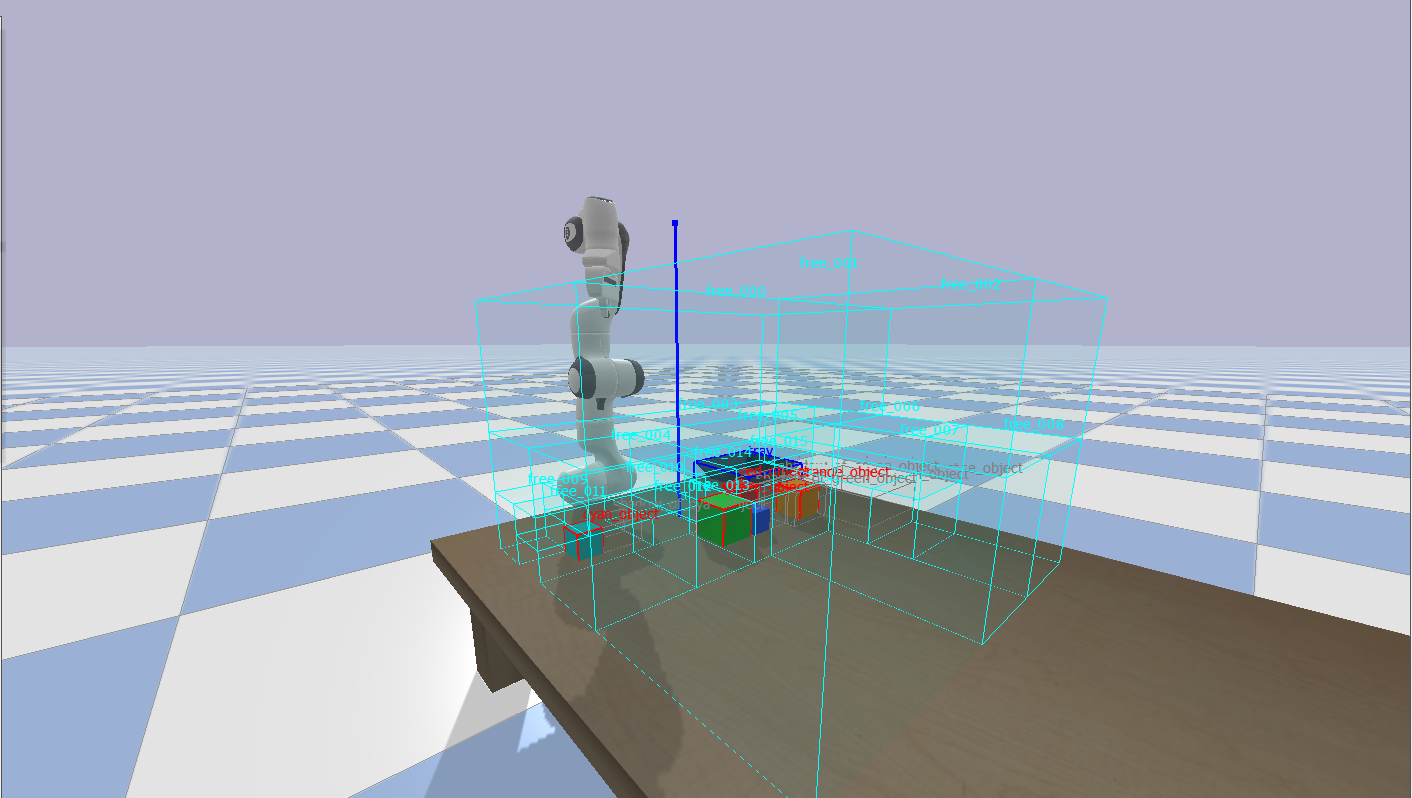
\includegraphics[height=2.5cm]{sim/partition_semantic.png} &
     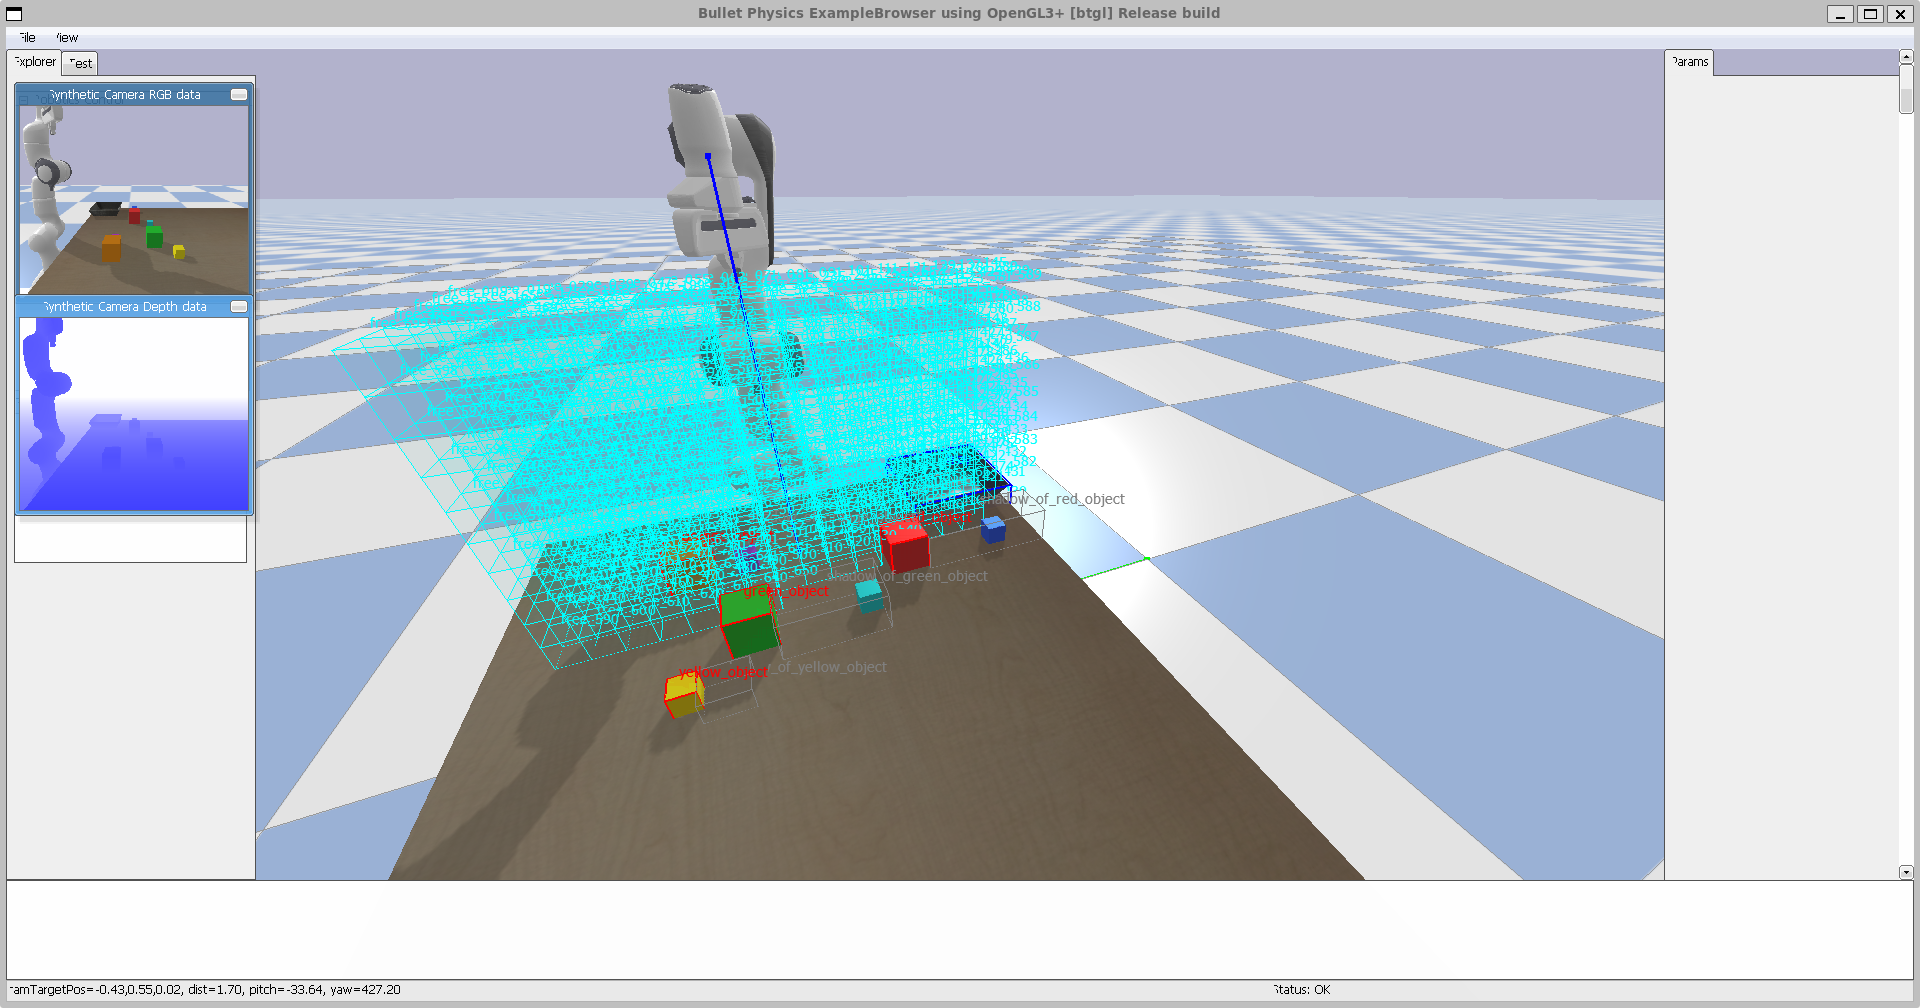
\includegraphics[height=2.5cm]{sim/partition_uniform.png} \\[1pt]
     {\scriptsize\color{gray}\textbf{semantic}} &
     {\scriptsize\color{gray}\textbf{uniform}} \\
   \end{tabular}
   \end{center}}
  \begin{itemize}
    \item<3-> \textbf{RQ2 (comparison):} how does deterministic POD-TAMP compare
          to a POMDP-based baseline (TAMPURA \rc{Curtis et al.}{Cur+24}) on the
          closest hidden-object task?
  \end{itemize}
  \medskip
  \onslide<4->{%
  {\color{i6blue}\bfseries Setup:} PyBullet + 7-DOF Franka Panda, one fixed camera,
  \textbf{oracle} perception; 3 goals $\times$ 3 difficulty levels $\times$ 30
  seeds, 1800\,s budget each. Oracle perception isolates the representation --- an
  ablation, not a benchmark win.}
\end{frame}

% --- E2. The three goals + difficulty axis ---
\begin{frame}{Experimental Evaluation: Tasks}
  \begin{columns}[T]
    \begin{column}{0.33\textwidth}
      \centering
      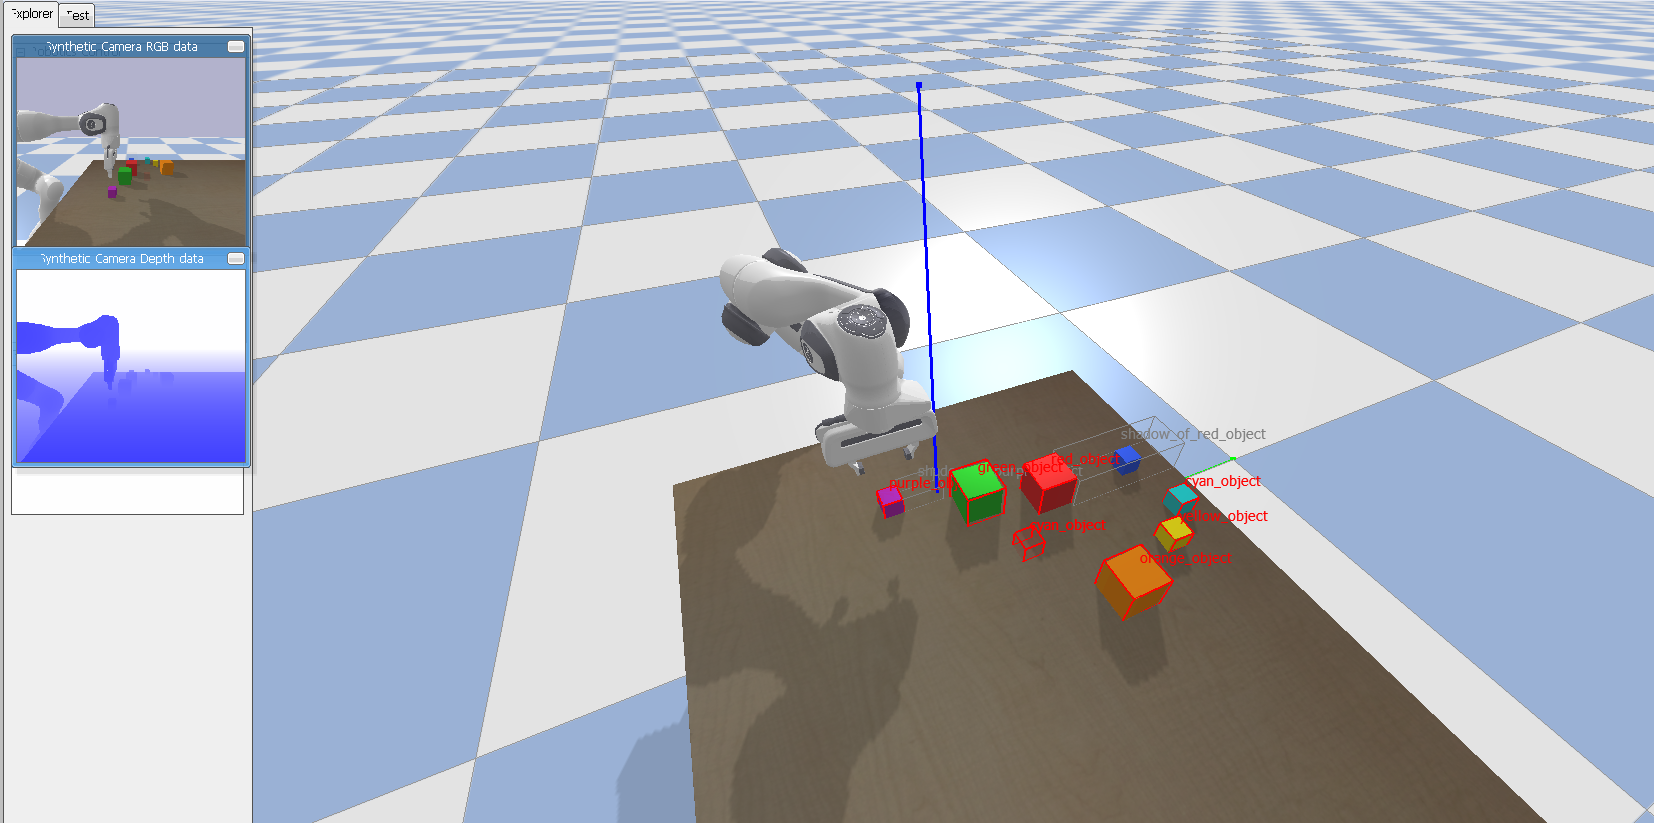
\includegraphics[width=\linewidth]{sim/task_holding.png}\\[2pt]
      {\footnotesize\color{gray}\texttt{holding}: retrieve a hidden target}
    \end{column}
    \begin{column}{0.33\textwidth}
      \centering
      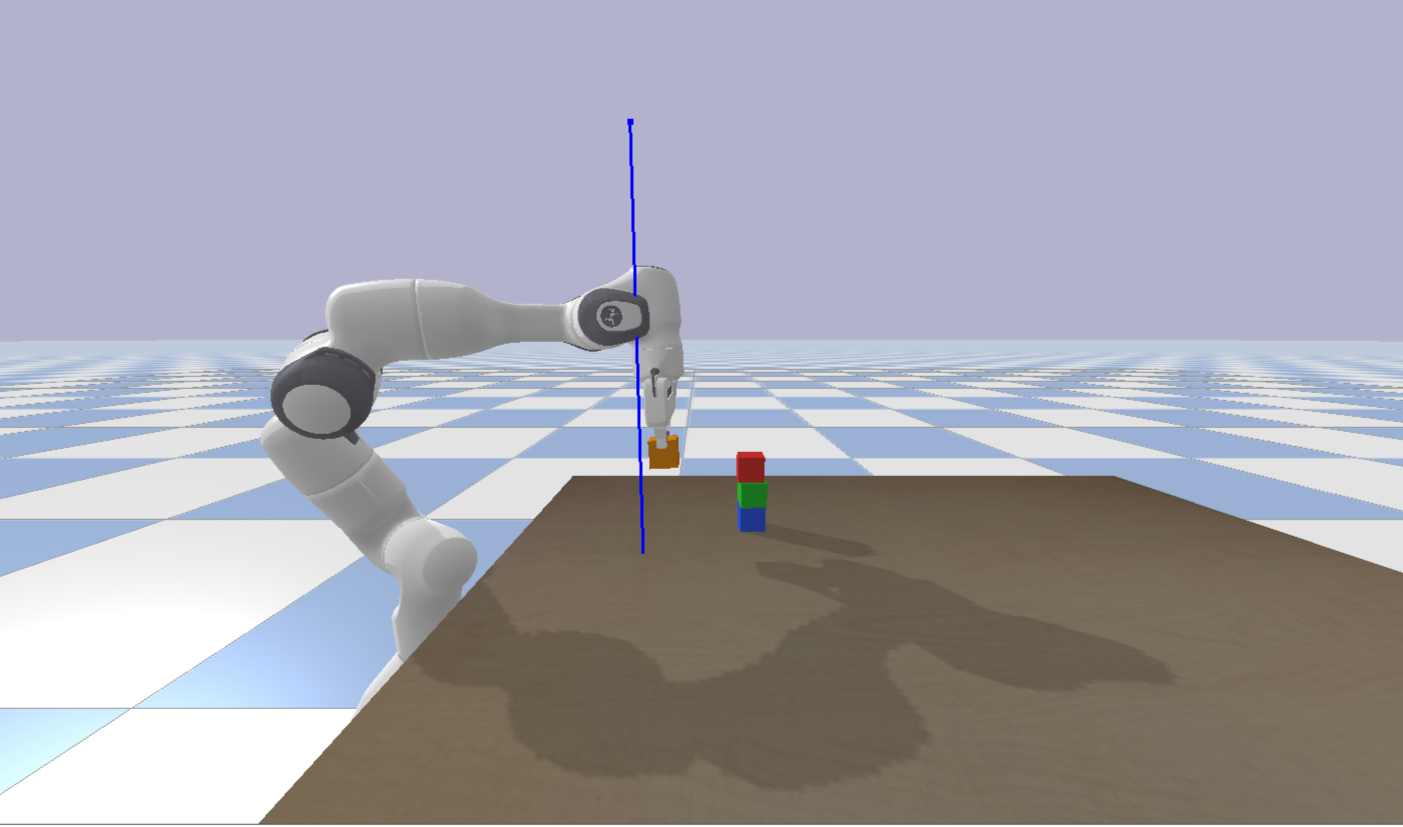
\includegraphics[width=\linewidth]{sim/task_stack.png}\\[2pt]
      {\footnotesize\color{gray}\texttt{stack}: build a tower to height $h$}
    \end{column}
    \begin{column}{0.33\textwidth}
      \centering
      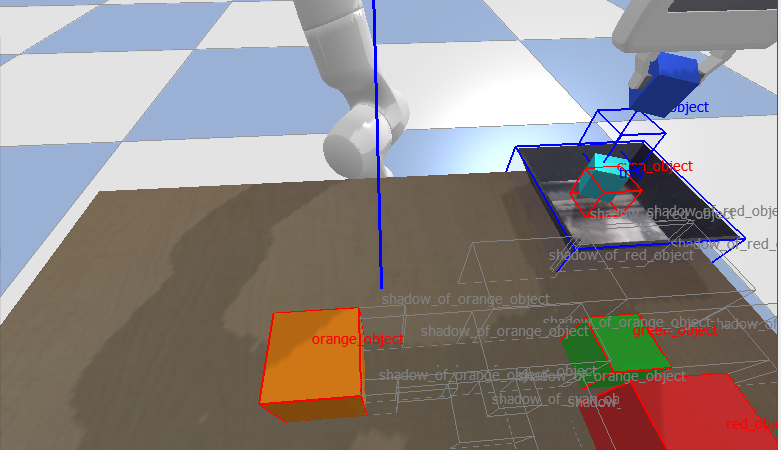
\includegraphics[width=\linewidth]{sim/task_tray.png}\\[2pt]
      {\footnotesize\color{gray}\texttt{find-and-tray-stack}: find, then stack on a tray}
    \end{column}
  \end{columns}
  \vspace{3mm}
  \pause
  \begin{itemize}
    \item Difficulty axis: number of occluders $n_\text{occ}\in\{2,3,4\}$ (search
          goals), or stack height $h\in\{2,3,4\}$ --- each adds shadow regions or
          tower layers
  \end{itemize}
\end{frame}

% --- E3a. The two partitions side by side: what the ablation compares ---
\begin{frame}{Results: Semantic vs Uniform Partition}
  \begin{columns}[T]
    \begin{column}{0.5\textwidth}
      \centering
      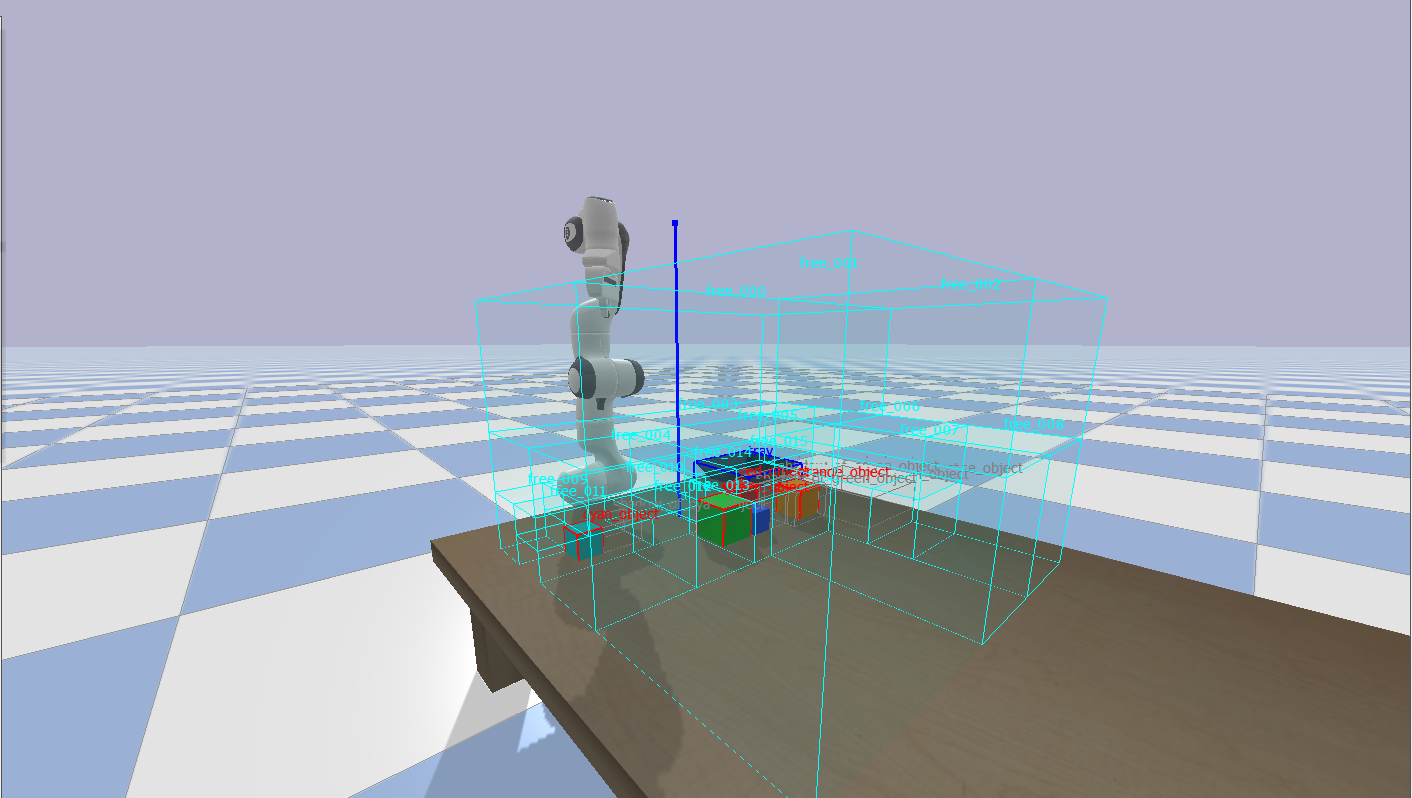
\includegraphics[width=\linewidth]{sim/partition_semantic.png}\\[2pt]
      {\footnotesize\color{gray}\textbf{semantic}: $\approx$22--38 task-relevant Boxels}
    \end{column}
    \begin{column}{0.5\textwidth}
      \centering
      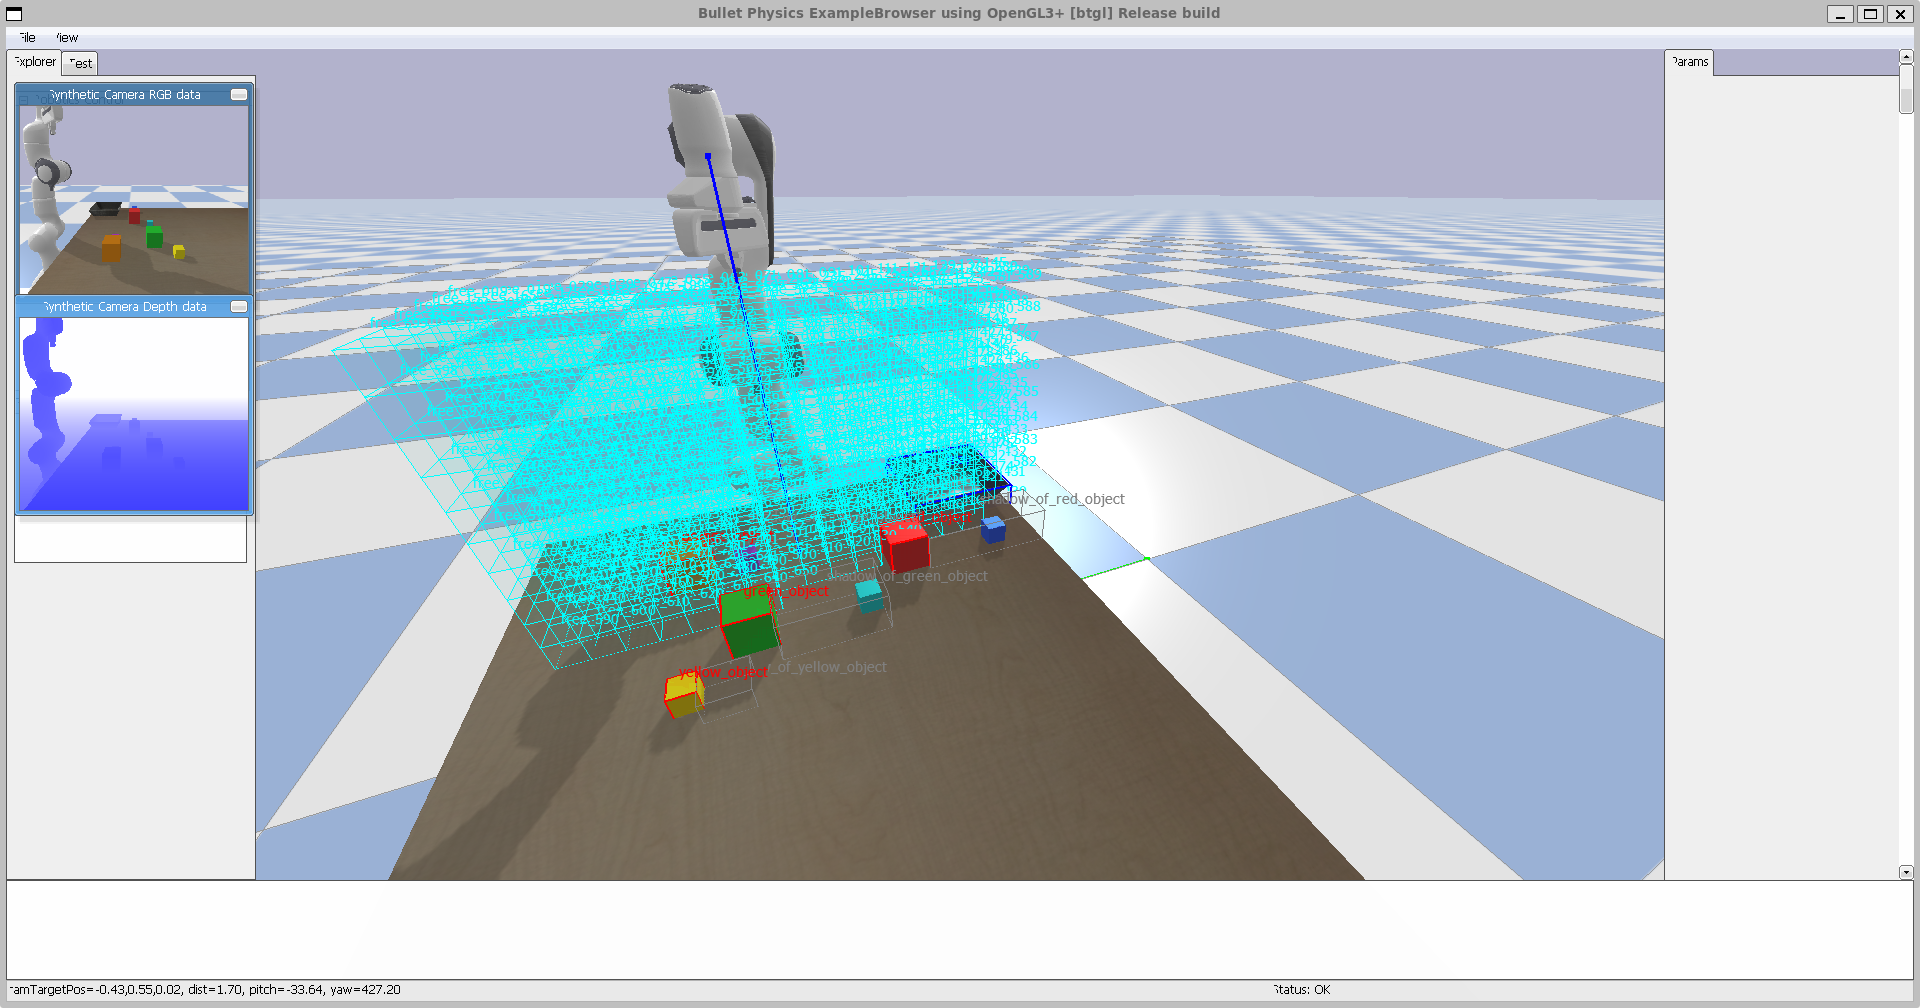
\includegraphics[width=\linewidth]{sim/partition_uniform.png}\\[2pt]
      {\footnotesize\color{gray}\textbf{uniform}: $\sim$300 fixed cells over the whole workspace}
    \end{column}
  \end{columns}
  \vspace{2mm}
  \centering
  {\footnotesize Same cell size, same planner --- the adaptive partition grounds
  and searches an order of magnitude fewer cells.}
\end{frame}

% --- E3b. Headline results table: semantic vs uniform ---
\begin{frame}{Results: Success and Planning Time}
  \vspace{2mm}
  \centering
  \small
  \begin{tabular}{llrr}
    \toprule
    goal & variant & success & mean plan time (s) \\
    \midrule
    find-and-tray-stack & \textbf{semantic} & \textbf{75.6\,\%} & \textbf{124.6} \\
                        & uniform           & 34.4\,\%          & 692.1 \\
    \midrule
    holding             & \textbf{semantic} & \textbf{65.6\,\%} & \textbf{134.3} \\
                        & uniform           & 47.8\,\%          & 438.5 \\
    \midrule
    stack               & \textbf{semantic} & \textbf{64.4\,\%} & \textbf{17.2} \\
                        & uniform           & 35.6\,\%          & 924.1 \\
    \bottomrule
  \end{tabular}
  \par\medskip
  \pause
  {\footnotesize Same planner, same cell size: the adaptive partition solves
  $\approx$1.4--2.2$\times$ more scenes, while planning several-fold to
  $\sim$50$\times$ faster.}
\end{frame}

% --- E4. Anytime solve rate + the compactness mechanism ---
\begin{frame}{Results: The Cost Gap}
  \begin{columns}[T]
    \begin{column}{0.6\textwidth}
      \centering
      
\includegraphics[width=\linewidth]{solved_vs_time_linear.png}\\[3pt]
      {\scriptsize\color{gray} \texttt{semantic+mbs0.05}: the same partition with a
       5\,cm minimum free-cell size (a resolution check) --- it overlaps
       \texttt{semantic}.}
    \end{column}
    \begin{column}{0.4\textwidth}
      \begin{itemize}[<+->]
        \item The adaptive partition \textbf{dominates at every budget};
              \texttt{uniform} starts later and plateaus lower
        \item \textbf{Mechanism:} $\approx$22--38 Boxels vs $\sim$300 free cells
              $\Rightarrow$ $\sim$300 vs 11k--14k grounded facts
        \item Fewer cells $\Rightarrow$ faster grounding $\Rightarrow$ more scenes
              finish in time
      \end{itemize}
    \end{column}
  \end{columns}
\end{frame}

% --- E5. Architectural comparison with TAMPURA ---
\begin{frame}{Results: Comparison with TAMPURA}
  \begin{columns}[T]
    \begin{column}{0.5\textwidth}
      \centering
      
\includegraphics[width=\linewidth]{tampura_wallclock_comparison.png}
    \end{column}
    \begin{column}{0.5\textwidth}
      \begin{itemize}[<+->]
        \item Rough \textbf{parity} end-to-end ($\approx$144\,s vs 166\,s per
              episode) and comparable reliability (65.6\,\% vs the $\geq$63\,\%
              its returns imply)
        \item The contrast is \emph{architectural}: deterministic
              knowledge-literal planning + replanning vs a \textbf{learned
              probabilistic MDP} solved with LAO*
        \item We hold occlusion as \textbf{symbolic state} --- line of sight is a
              planning condition; TAMPURA keeps it sub-symbolic
        \item Not a benchmark win: different environments, same hardware
      \end{itemize}
    \end{column}
  \end{columns}
\end{frame}

% ===========================================================================
% 6. Discussion
% ===========================================================================
\section{Discussion}

\begin{frame}{Discussion: Limitations}
  \begin{itemize}[<+->]
    \item \textbf{Oracle perception:} a ground-truth pose detector, no learned
          module and no sensor noise --- deliberate, to isolate the representation
    \item \textbf{One fixed camera:} the robot never reasons about \emph{where to
          look}
    \item \textbf{Simplified manipulation}: top-down grasps, welded grip, a
          hardcoded post-place lift
    \item \textbf{Box-shaped shadows under-cover the hidden region:} the volume an
          object occludes is really a cone, so a target tucked into the uncovered
          part gets no Boxel to sense --- our most common failure
    \item \textbf{Bounded give-up:} on a permanently blocked shadow the planner
          eventually stops searching --- unsound, since the target may still be
          reachable (we determinize-and-replan, not full contingent POD)
  \end{itemize}
\end{frame}

\begin{frame}{Discussion: Future Work \& Takeaway}
  \begin{itemize}[<+->]
    \item \textbf{Future work:}
      \begin{itemize}[<+->]
        \item[\emoji{robot}] a real-robot Franka study
        \item[\emoji{brain}] a learned detector on the RGB-D images, dropped in
              behind the same detection interface
        \item[\emoji{camera}] active sensing with a robot-mounted camera (a
              where-to-look stream)
        \item[\emoji{package}] recurse into concave geometry (containers, cupboards)
        \item[\emoji{puzzle-piece}] a full semantic free-space merge
      \end{itemize}
  \end{itemize}
  \vspace{2mm}
  \onslide<+->{%
  {\color{i6blue}\textbf{Takeaway:}} making occlusion an explicit, named piece of
  symbolic state lets a simple \emph{deterministic} planner do partially observable
  TAMP --- reasoning about where to look --- without learning a probabilistic policy.}
\end{frame}

% ===========================================================================
% Closing
% ===========================================================================
\begin{frame}{Summary}
  \begin{itemize}
    \item \textbf{Problem:} TAMP under occlusion --- the robot must decide
          \emph{where to look}, but a dense voxel belief is too large to plan over
    \item \textbf{Idea:} \textbf{Boxels} --- task-relevant box-shaped cells
          (object\,/\,shadow\,/\,free) that put the structure of space into the
          symbolic state
    \item \textbf{Method:} a deterministic POD-TAMP planner reasons over Boxels
          with Know-If fluents; optimistic sensing $+$ replanning resolve the
          unknown
    \item \textbf{Result:} an order of magnitude fewer cells $\Rightarrow$ far more
          cluttered scenes solved than a uniform grid; at parity with TAMPURA,
          without a learned probabilistic policy
  \end{itemize}
  \vfill
  \begin{center}
    {\color{i6blue}\Large\bfseries Thank you!}\quad
    {\color{gray}\large Questions?}
  \end{center}
  \vspace{2mm}
\end{frame}

% ===========================================================================
% Backup slides (for Q&A)
% ===========================================================================
\appendix
\setcounter{framenumber}{0}

% References. Hand-typed to match the inline \rc{..}{Key} labels (the deck carries
% no biblatex bibliography); keys/details mirror thesis/resources/references.bib.
\begin{frame}{References}
  \scriptsize
  \begin{columns}[T]
    \begin{column}{0.49\textwidth}
      {\color{i6blue!60}\textbf{[Bon+11]}} Bonet, B. \& Geffner, H. \emph{Planning
       under Partial Observability by Classical Replanning.} IJCAI, 2011.\par\smallskip
      {\color{i6blue!60}\textbf{[Cur+24]}} Curtis, A.\ et al. \emph{Partially
       Observable Task and Motion Planning with Uncertainty and Risk Awareness.}
       arXiv:2403.10454, 2024.\par\smallskip
      {\color{i6blue!60}\textbf{[Gar+18]}} Garrett, C.\,R., Lozano-P\'erez, T. \&
       Kaelbling, L.\,P. \emph{PDDLStream: Integrating Symbolic Planners and
       Blackbox Samplers.} arXiv:1802.08705; ICAPS, 2020.\par\smallskip
      {\color{i6blue!60}\textbf{[Gar+20]}} Garrett, C.\,R.\ et al. \emph{Online
       Replanning in Belief Space for Partially Observable Task and Motion
       Problems.} ICRA, 2020.\par\smallskip
      {\color{i6blue!60}\textbf{[Gef+13]}} Geffner, H. \& Bonet, B. \emph{A Concise
       Introduction to Models and Methods for Automated Planning.} Morgan \&
       Claypool, 2013.\par\smallskip
      {\color{i6blue!60}\textbf{[Hor+13]}} Hornung, A.\ et al. \emph{OctoMap: An
       Efficient Probabilistic 3D Mapping Framework Based on Octrees.} Autonomous
       Robots, 2013.\par\smallskip
      {\color{i6blue!60}\textbf{[Kae+98]}} Kaelbling, L.\,P., Littman, M.\,L. \&
       Cassandra, A.\,R. \emph{Planning and Acting in Partially Observable
       Stochastic Domains.} Artificial Intelligence, 1998.
    \end{column}
    \begin{column}{0.49\textwidth}
      {\color{i6blue!60}\textbf{[Kuf+00]}} Kuffner, J.\,J. \& LaValle, S.\,M.
       \emph{RRT-Connect: An Efficient Approach to Single-Query Path Planning.}
       ICRA, 2000.\par\smallskip
      {\color{i6blue!60}\textbf{[Mol+20]}} Molina, D., Kumar, K. \& Srivastava, S.
       \emph{Learn and Link: Learning Critical Regions for Efficient Planning.}
       ICRA, 2020.\par\smallskip
      {\color{i6blue!60}\textbf{[Pan+24]}} Pan, T., Shome, R. \& Kavraki, L.\,E.
       \emph{Task and Motion Planning for Execution in the Real.} IEEE Trans.\
       Robotics, 2024.\par\smallskip
      {\color{i6blue!60}\textbf{[Pet+02]}} Petrick, R.\,P.\,A. \& Bacchus, F.
       \emph{A Knowledge-Based Approach to Planning with Incomplete Information and
       Sensing.} AIPS, 2002.\par\smallskip
      {\color{i6blue!60}\textbf{[Yoo+07]}} Yoon, S.\,W., Fern, A. \& Givan, R.
       \emph{FF-Replan: A Baseline for Probabilistic Planning.} ICAPS, 2007.\par\smallskip
      {\color{i6blue!60}\textbf{[Zha+25]}} Zhao, L.\ et al. \emph{Seeing is
       Believing: Belief-Space Planning with Foundation Models as Uncertainty
       Estimators.} arXiv:2504.03245, 2025.
    \end{column}
  \end{columns}
\end{frame}

\begin{frame}{Backup: Representation Compactness}
  \begin{columns}[T]
    \begin{column}{0.62\textwidth}
      \centering
      
\includegraphics[width=\linewidth]{boxel_count_breakdown__holding.png}
    \end{column}
    \begin{column}{0.38\textwidth}
      \begin{itemize}
        \item Adaptive: $\approx$22--38 Boxels in total
        \item \texttt{uniform}: $\sim$300\,+ free-space cells alone
        \item An order of magnitude fewer cells to ground and search
      \end{itemize}
    \end{column}
  \end{columns}
\end{frame}

\begin{frame}{Backup: Free-Space Resolution}
  \centering
  
\includegraphics[width=0.8\textwidth]{boxel_count_vs_resolution.png}\\[3pt]
  {\footnotesize The partition is \textbf{insensitive} to the free-space leaf
   size: flat from 5\,cm to the auto setting; only the extreme 1\,mm floor breaks
   feasibility (too fine to plan within budget).}
\end{frame}

% Moved out of the main Results flow (kept for Q&A): scaling with clutter.
\begin{frame}{Backup: Scaling with Clutter}
  \begin{columns}[T]
    \begin{column}{0.5\textwidth}
      \centering
      
\includegraphics[width=\linewidth]{success_rate_vs_n_occluders__holding.png}
    \end{column}
    \begin{column}{0.5\textwidth}
      \centering
      
\includegraphics[width=\linewidth]{success_rate_vs_n_occluders__find-and-tray-stack.png}
    \end{column}
  \end{columns}
  \vspace{1mm}
  {\footnotesize \textbf{More occluders do not break the adaptive partition:} it
   stays well above \texttt{uniform} at every clutter level, and even rises at the
   densest scenes.}
  \par\smallskip
  {\scriptsize\color{gray} Orange is \texttt{semantic+mbs0.05} --- the same
   partition with a 5\,cm floor on free-cell size (a resolution check); it tracks
   \texttt{semantic}. \texttt{stack} instead scales with tower \emph{height}, not
   clutter --- a manipulation limit, not the planner.}
\end{frame}

\begin{frame}{Backup: Failure Modes}
  \centering
  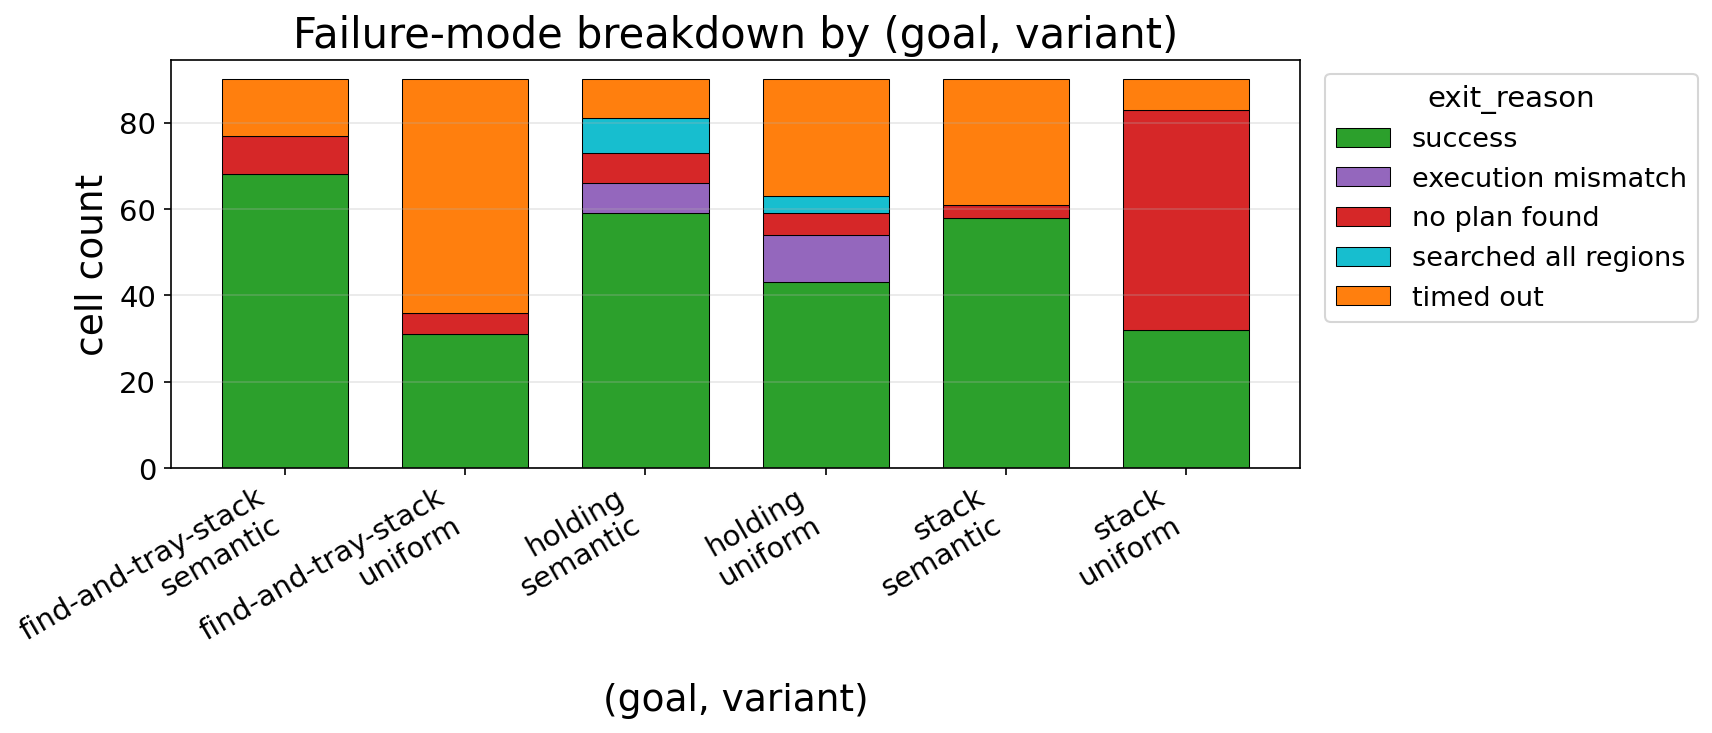
\includegraphics[width=0.92\textwidth]{failure_modes_sem_uni_detailed.png}\\[4pt]
  {\footnotesize Exit reason per (goal, variant), 90 runs each. \textbf{uniform}
   fails mostly by \emph{timing out} (and \emph{no plan found} on \texttt{stack}):
   it cannot ground and search $\sim$300 cells within budget. \textbf{semantic}'s
   residual failures are fewer, split across \emph{timed out}, \emph{search
   exhausted} (target outside every box-shaped shadow), and \emph{false success}
   (a physics mismatch at execution).}
\end{frame}

\end{document}
